%!TEX root = thesis.tex


%
%==========================================================================================
%
\chapter{Ambient Assisted Living Domain}
\label{chap:confidence}

\index{activities of daily living, ADL}
\index{ambient intelligence, AmI}
\index{daily-living dynamics}
Analyzing  daily-living behavior is an important approach to assessing the wellbeing of an elderly person living at home alone. This chapter presents an approach to monitoring an individual in the home environment by an ambient-intelligence system to detect daily living pattern anomalies. It utilizes the proposed unified framework to recognize activities, extract spatio-activity behavior signatures, and apply an outlier-detection method to classify the individual's daily patterns, regardless of the cause of the problem, be it physical or mental. Experiments indicate that the proposed solution successfully discriminates between healthy person behavior patterns and those of a person with health problems.

\section{Introduction and Background}
\label{sec:introduction}

%
%Set context and motivate the overall field of study 
%
\index{ambient assisted living, AAL}
\index{ambient intelligence, AmI}
Recent years have seen increased interest in the deployment of systems for ambient assisted living (AAL) \citep{Augusto2012}, including remote eldercare \citep{Kaluza2010Agentbased}, smart homes \citep{Cook}, surveillance \citep{Dore}, etc. Whereas some of these systems can be tele-operated, the AAL community strives to design systems that monitor a person autonomously and act in the case of an emergency, warning or suggestion, such as fall detection~\citep{Bourke, Lustrek2009Behavior}. Our study targets persons in the home environment; that is, a male or female senior citizen, who does not need intensive care or assistance in day-to-day living, but accepts an ambient-intelligence (AmI) system to improve their health, safety, and well-being. The main issue is anomaly detection in the monitored person's daily behavior.

%
% Provide a concrete problem statement 
% - person-friendly HW
% - accurate activity recognition
% - uknown activites of DL
% - adaptation to each person
%
A predominant approach consists of three components: a sensor system, an activity-recognition model, and a daily behavior analysis~\citep{Choudhury06towards}. There are several challenges to constructing such a system. First, the person must be monitored with sensors that are not obtrusive, invasive or privacy-violating, yet are precise enough to address the second challenge, which is an accurate activity recognition model. An underlying recognition model needs to detect a wide variety of activities performed differently under different environmental conditions and across many individuals. Third, we have no knowledge about the exact plans and schedules a person may follow during the day. In addition, the system should adapt to each specific person while deployed at the person's home.

%
% Explain why previous work fails in addressing the problem statement 
%
%
% Explain our ideas and why they are new and overcome the limitations of para 3 
%
In remote eldercare, the AAL systems use a wide variety of sensors, such as vision systems~\citep{Fabien}, inertial sensors~\citep{Bourke} and embedded sensors~\citep{Lymberopoulos, Monekosso}. While some sensors might violate privacy issues, for example, a camera, others do not provide additional location context, for example, inertial sensors, or rich information required for accurate activity and posture recognition, for example, embedded sensors. Daily behavior analysis may focus on recognizing or describing exact schedules and assumes that the person will follow them. Another approach relies on either observers, that is, a nurse who periodically observes an elderly person, or on self-reporting, that is, having people complete an activity report at the end of the day. Both ways of reporting have limited accuracy and usefulness due to the aggregation in time, forgetfulness, and misreporting (intentional or unintentional). 

In contrast to related work discussed in Section~\ref{related:behavior:transaction}; that is, fuzzy-association analysis \citep{Lee04daily}, Apriori algorithm combined with Markov chain \citep{Lymberopoulos}, and HMMs \citep{Monekosso}, this chapter uses a localization system (in other publications, accelerometers are more often used) with wireless body-worn tags (described in Section \ref{sec:experiments}), while low-level activity recognition is performed with a SVM classifier. These two modules were developed within the Confidence system \citep{Kaluza2010Agentbased}. This chapter focuses on the third component; that is, daily patterns analysis that detects behavior changes indicating an early discovery of a potential health problem, such as a person visiting a toilet unusually often. In contrast to related work, which mainly dealt with a description of high-level activities, our method focuses on activity dynamics; by contrast to Markov models, it explores the relations between spatial information and activities. %The method detects anomalous behavior regardless of the cause.
The method is general in the sense that it detects unusual behavior regardless of the cause, be it illness of any kind, any physical or mental degradation or even an outside cause, for example, being locked in a room. 

%The central hypothesis is that daily movement patterns can be learned for a specific person and the anomalous behavior can be detected when compared to the learned patterns.
%We propose a presentation that aggregates a daily activity log into a \textit{spatio-activity matrix}. It can be used to visualize the person's daily dynamics. For automatic detection with machine learning we propose a method for evaluating the behavior anomalousness based on principal component analysis (PCA) for feature extraction and the local outlier factor algorithm (LOF)~\cite{Breunig00lof} for detecting anomalous behavior patterns. 


%
% How did you evaluate your new ideas and what were some key results that should motivate the reader to read the rest of the paper
%
%We deployed the system in a lab organized as a near-realistic home apartment of about $25$~$m^2$ and equipped with the Ubisense localization system~\cite{Ubisense}. The activity-recognition model trained on several persons was able to achieve a better than 87\% accuracy in recognizing the activities of a new person~\cite{Kaluza2010Agentbased}. We experimentally tested our new approach in multiple episodes with several persons involving regular behavior and behavior when a person does not feel well. The experiments showed that the proposed method was able to discover all clearly deviating behavior patterns.

%The rest of the paper is structured as follows. Section~\ref{sec:background:related} reviews the related work and delimits this work. Next, Section~\ref{sec:overview} introduces the general structure of the system and describes the deployed sensors and activity recognition method. The main contribution of this work is presented in Section~\ref{sec:ba}, where the method for analysis of daily-living dynamics is proposed. Section~\ref{sec:experiments} presents the experimental setup and provides experimental evaluation, while Sections~\ref{sec:discussion} and \ref{sec:conclusion} close the paper with discussion and conclusion.




%%%%%%%%%%%%%%%%%%%%%%%%%%%%%%%%%%%%%%%%%%%%%%%%%%%%%%%%%%%%%%%%%%%%%%%%%%%%%%%%
\section{System Architecture}
\label{sec:overview}
%
%Overview of the Approach
%
\index{activity recognition pipeline}
\index{activity recognition}
\index{unified framework}
The instantiated unified framework is presented in Figure~\ref{fig:scheme}. % consists of 10 layers. % the learning (left-hand side) and recognizing (right-hand size) phases. Both phases, however, share some steps. 
First, raw sensor readings are obtained from the environment at each time step. Next, the activity recognition pipeline (ARPipe) is deployed as described in Chapter~\ref{chap:activity_recognition}. It prepocesses observation vectors to reduce noise, and compute additional features.  Next, an activity recognition algorithm classifies the observation vector at time $t$ into one of the activities an individual can perform; for example, \emph{walking, sitting, lying}. The output is a behavior trace consisting of activities and the places where they were performed. The trace is converted to a spatio-activity matrix, which is afterwards reduced with principal value decomposition. Finally, the LOF algorithm compares the behavior to an historical behavior signature database.

\begin{figure*}[!ht]
\centering
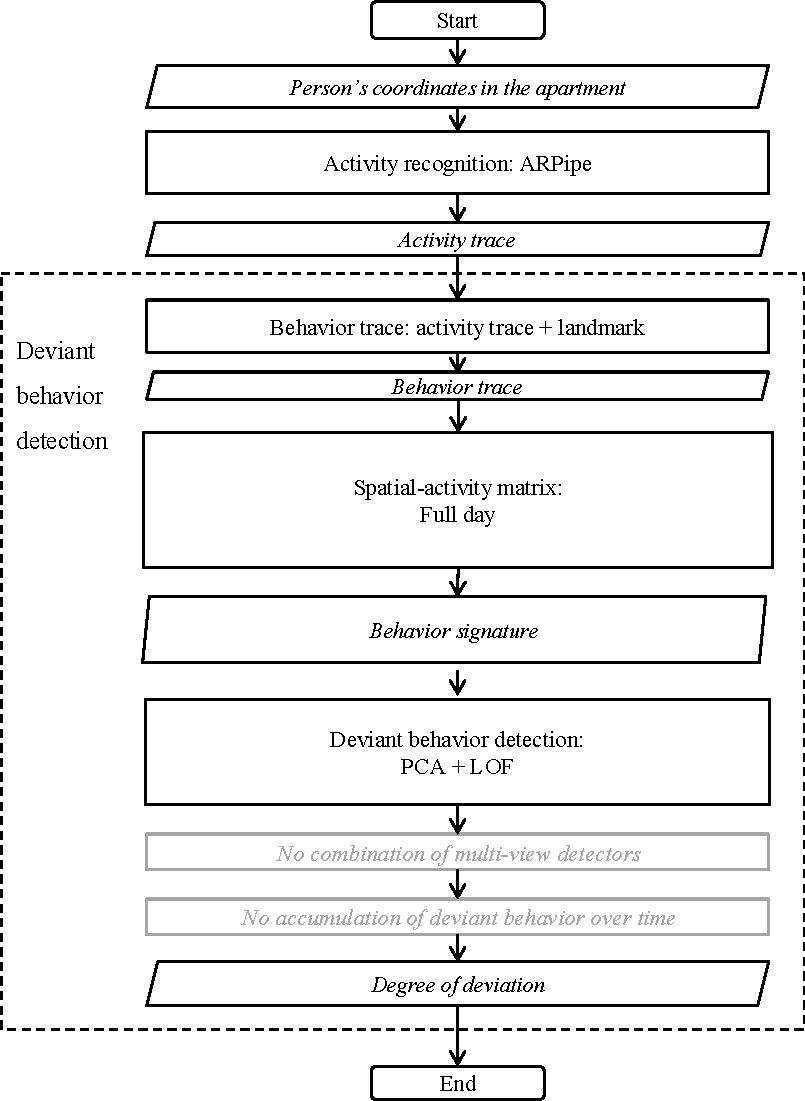
\includegraphics[width=0.8\textwidth]{chap_AAL/stack-AAL.pdf}
\caption{Flowchart of the instantiated unified framework for analyzing daily-living dynamics.}
\label{fig:scheme}
\end{figure*}

\subsection{Sensors and Observations}
\label{sec:overview:data}

We deployed the system in a lab organized as a home apartment, equipped with the Ubisense localization system~\citep{Ubisense}, which allows local positioning by tracking a set of tags attached to a person. The tags were placed at the following locations on the body, as shown in Figure~\ref{fig:tags}: chest, waist, left and right ankle. Each observation vector consists of the absolute $x$, $y$, and $z$ coordinates. 
The observation sequence passed to the next level was a movement trajectory of all the tags in time interval $1 \leq t \leq T$:
$$\mathbf{X}=\{[x_{tag}, y_{tag}, z_{tag}, \cdots]_t | tag \in \{chest, waist, l\_ankle, r\_ankle\}, 1 \leq t \leq T\}.$$

\begin{figure}[!ht]
\centering
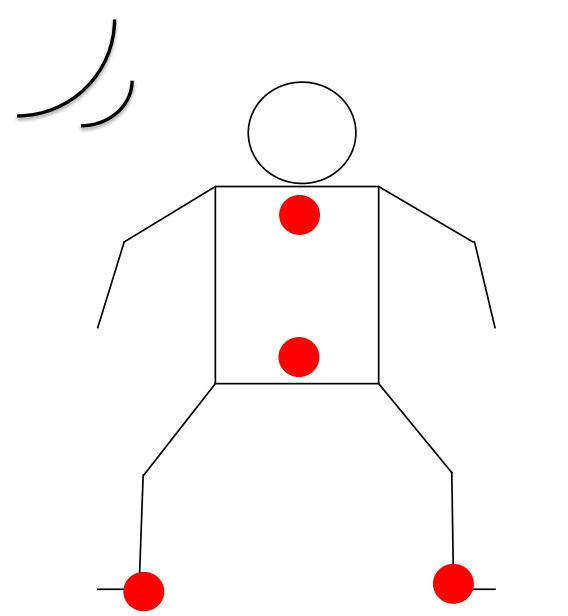
\includegraphics[width=0.3\textwidth, bb=0 0 370 420]{chap_AAL/tags.jpg}
\caption{Ubisense tag placement.}
\label{fig:tags}
\end{figure}



\subsection{Activity Recognition Pipeline}
\label{sec:overview:ar}

\index{activity recognition pipeline}
The raw sensor data are further processed with ARPipe as described in Chapter~\ref{chap:activity_recognition}. First, a median filter is applied to remove the impulsive noise. Next, an iterative constrain satisfaction method that enforces human body constraints between the measured tag positions is applied. Finally, Kalman's filter estimates additional parameters, such as tag velocity.

Activity recognition is performed in three steps. First, we extract tag attributes, such as the $z$ coordinates, all tag velocities, the absolute distances, and the $z$ direction distances between all the tag pairs. Activity recognition omits $x$ and $y$ coordinates because, from the activity-classification point of view, the location of an activity is not important. However, the $x$ and $y$ coordinates are essential for any daily living pattern analysis.

\index{canonical representation}
Second, person postures are classified into one of the following atomic activities: $\mathbb{A}=\{walking, sitting, lying\}$. The feature vector uses canonical representation with window length $W=10$. A new feature window is then obtained after every update, thus overlapping with the previous one, and provides instant classification for each observation vector. We have tested a variety of machine-learning algorithms \citep{Lustrek2009Fall}, including C4.5 decision trees, na{\"i}ve Bayes, SVM, k-NN, bagging, AdaBoost, etc., with SVM offering the highest classification accuracy.

\index{spurious activity transitions}
Third, activity recognition errors that produced spurious activity transitions were reduced using the HMMs \citep{Rabiner1989} as described in Section~\ref{sec:ar:spurious}. Preliminary results indicated that HMMs are superior compared to sequential grammar-based classifiers \citep{Kaluza09Reducing}. The HMM was initialized with $\mathbb{A}=\{walking, sitting, lying\}$ observation symbols, three internal hidden states corresponding to activities, the initial state transition probability $\delta_{ij} = 1/3$, the initial state probability $\pi_i=1/3$, and the output symbol distribution in state $\nu_j(k) = 1$ if $k=j$, otherwise $\nu_j(k)=0$. The parameters were estimated with the Baum-Welch method using $50$ iterations on the training data. The second phase, which finds the optimal hidden state transitions according to the observation sequence, was performed with the Viterbi algorithm. 


%\subsection{Behavior Analysis}
%\label{sec:overview:ba}


%%%%%%%%%%%%%%%%%%%%%%%%%%%%%%%%%%%%%%%%%%%%%%%%%%%%%%%%%%%%%%%%%%%%%%%%%%%%%%%%
\subsection{Behavior Analysis}
\label{sec:ba}

First, the behavior trace is constructed using $\tuple{activity, room}$ tuples. The apartment was divided into logical areas $\mathbb{S}=\{lounge, bedroom, kitchen, toilet\}$ and $(x_{waist},y_{waist})_t$ coordinates were used to determine the area at time step $t$. Then, the behavior trace $\mathbf{b}=\{(a, s)_t|1\leq t \leq T\}$ was passed to the next level.

\index{local outlier factor, LOF}
Behavior signatures were constructed using the spatio-activity matrix approach introduced in Chapter~\ref{chap:signatures} using Algorithm~\ref{alg:SA_matrix}. The matrix dimensionality was further reduced with PCA. Finally, the LOF algorithm \citep{Breunig00lof} assigned each behavior signature an outlier degree, called the local outlier factor (LOF) of a vector. Vectors with a high LOF have local densities smaller than their neighborhood and typically represent stronger outliers, unlike vectors belonging to uniform clusters that tend to have lower LOF values. 

More formally, assume that $\mathcal{B}_T=\{\mathbf{b}_i | 1 \leq i \leq L\}$ is a dataset of behavior traces. First, for each behavioral trace $\mathbf{b}_i$, we compute the spatio-activity matrix $\mathbf{M}_i$ using Algorithm~\ref{alg:SA_matrix}. Next, we compute the principal component vector $\mathbf{m}_i$ (Equations~\ref{eq:PCA-1}--\ref{eq:PCA-4}), and add vector $\mathbf{m}_i$ to a new behavior signature dataset $\mathcal{B}$. Next, for each vector $\mathbf{m}_i$, we compute the $k\_dist_i$ as the distance to the $k^{th}$ nearest neighbor of $\mathbf{m}_i$,  then compute the reachability distance for each vector $\mathbf{m}_i$ with respect to the vector $\mathbf{m}_j$, where $d(\mathbf{m}_i,\mathbf{m}_j)$ is the Euclidean distance from $\mathbf{m}_i$ to $\mathbf{m}_j$, and compute the local reachability density $lrd_i$ of the vector $\mathbf{m}_i$ as the inverse of the average reachability distance based on the $k$ nearest neighbors of the vector $\mathbf{m}_i$. Finally, we compute the $LOF_i$ of the vector $\mathbf{m}_i$ as the ratio of the average local reachability density of $\mathbf{m}_i$'s  $k$ nearest neighbors and the local reachability density of the vector $\mathbf{m}_i$.

\index{detector}
\index{local outlier factor, LOF}
\begin{algorithm}
\caption{Anomaly detection.}
\label{alg:LOF}
\begin{algorithmic}
\REQUIRE set of behavior traces $\mathcal{B}_T=\{\mathbf{b}_i | 1 \leq i \leq L\}$, number of $k$ nearest neighbors
\ENSURE outlier degree for each behavior trace $LOF_i$
\STATE $\mathcal{B} \gets \{\}$
\FOR {$\mathbf{b}_i \in \mathcal{B}_T$}
	\STATE $\mathbf{M}_i \gets spatial\_activity\_matrix(\mathbf{b}_i)$
	\STATE $\mathbf{m}_i \gets PCA(\mathbf{M}_i)$
	\STATE $\mathcal{B} \gets \mathcal{B} \cup \mathbf{m}_i $
\ENDFOR
\FOR {$\mathbf{m}_i \in \mathcal{B}$}
	\STATE $k\_dist_i \gets k\_distance(\mathbf{m}_i)$
	\FOR{$\mathbf{m}_j \in \mathcal{B}, \mathbf{m}_j \neq \mathbf{m}_i$}
		\STATE $r\_dist_{i,j} \gets max(d(\mathbf{m}_i, \mathbf{m}_j), k\_dist_j))$
	\ENDFOR
	\STATE $lrd_i = {k \over { \sum_{\mathbf{m}_j\in kNN(\mathbf{m}_i)}{r\_dist_{i, j}}}}$
	\STATE $LOF_i \gets { {1 \over k}{{ \sum_{\mathbf{m}_j\in kNN(\mathbf{m}_i)}{lrd_j}}} \over lrd_i}$
\ENDFOR
\end{algorithmic}
\end{algorithm}



%
%==========================================================================================
%
\section{Experimental Evaluation}
\label{sec:experiments}

%\subsection{Experimental Setup}
%\label{sec:experimental-setup}
For the prototype deployment we organized a room as an apartment of about~$25$~$m^2$. The apartment was equipped with a bed, a few chairs and tables, and divided into four logical areas: a kitchen, where a person can prepare a meal; a sleeping area; a lounge, where a person can eat a meal, watch TV, write a letter, etc.; and a toilet.



\subsection{Activity Recognition}
\label{sec:experiments:activities}
To build an activity recognition model, we recorded five members of our department. Each participant was recorded performing various activities in three episodes lasting approximately 15--20 minutes each. In total, there were around four hours of recordings. The scenario details are available in \cite{Kaluza2010Agentbased}.

The activity recognition confusion matrix presented in Table~\ref{tab:actRecognition} was obtained with a {\it leave-one-person-out} validation. The left-hand column shows the correct-activity label, and the top row shows the assigned label. The overall classification accuracy is $87.52$\%.

\begin{table}[h!]
\centering
\caption{Confusion matrix for activity recognition. The overall accuracy is $87.52$\%.}
\begin{tabular}{lcccc}
\toprule
True / Labeled [\%] & Lying & Sitting & Standing  \\
\hline
Lying    & 98.99& 0.93& 0.08  \\
Sitting  & 1.67& 67.71& 30.62 \\
Standing & 0.85& 3.27& 95.88 \\
\toprule
\end{tabular}
\label{tab:actRecognition}
\end{table}




\subsection{Anomalous Behavior Detection}
\label{sec:experiments:behavior}

We performed two experiments as follows: the first experiment condensed a full day of activities into scenarios of around half an hour each, while the second test analyzed person behavior in the office for a period of one month.


\begin{figure}[h!t]
 \centering
 \subfloat[Normal day 1]{\label{fig:day-n-1}
 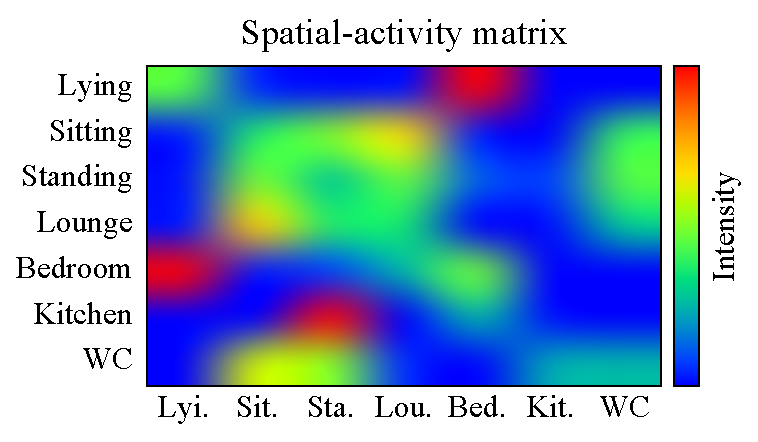
\includegraphics[width=0.50\textwidth]{chap_AAL/matrix-b-3}}
 \subfloat[Normal day 2]{\label{fig:day-n-2}
 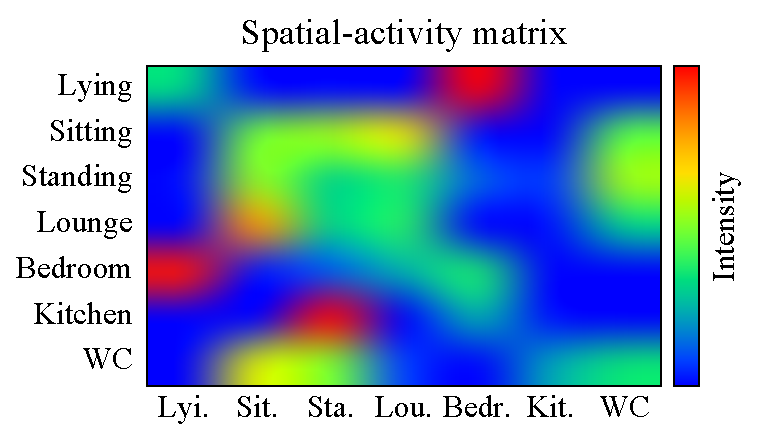
\includegraphics[width=0.50\textwidth]{chap_AAL/matrix-b-4}}

 \subfloat[Normal day 3]{\label{fig:day-n-3}
 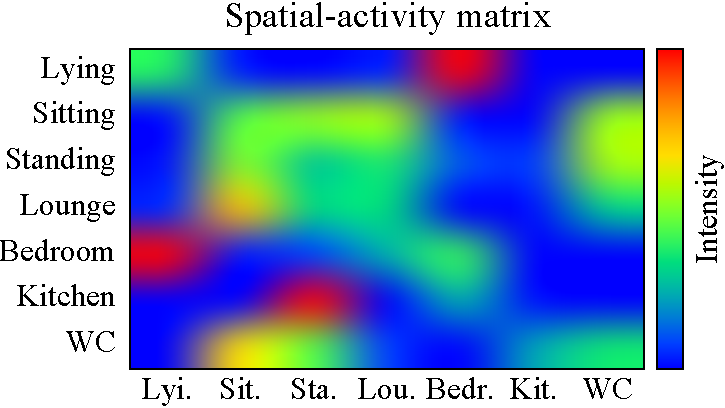
\includegraphics[width=0.50\textwidth]{chap_AAL/matrix-b-5}}
 \subfloat[Normal day 4]{\label{fig:day-n-4}
 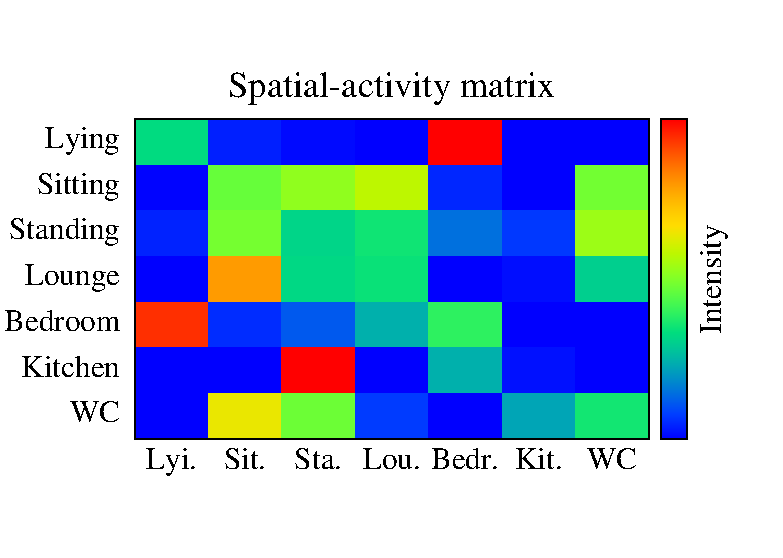
\includegraphics[width=0.50\textwidth]{chap_AAL/matrix-b-6}}

 \subfloat[Slow day]{\label{fig:day-c-1}
 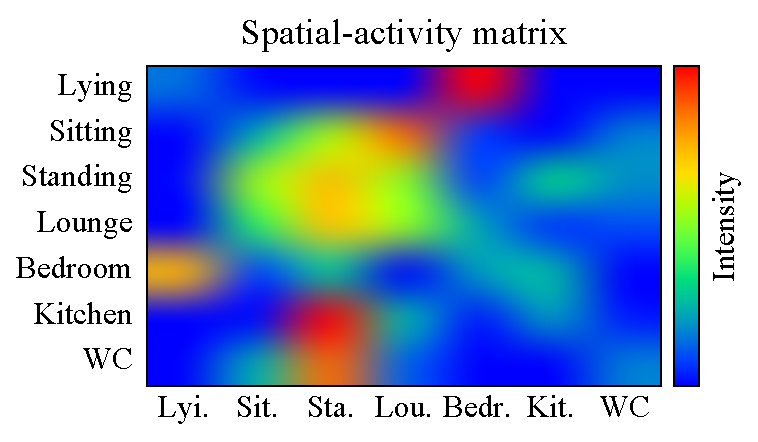
\includegraphics[width=0.50\textwidth]{chap_AAL/matrix-b-c-1}}
 \subfloat[Limping day]{\label{fig:day-c-2}
 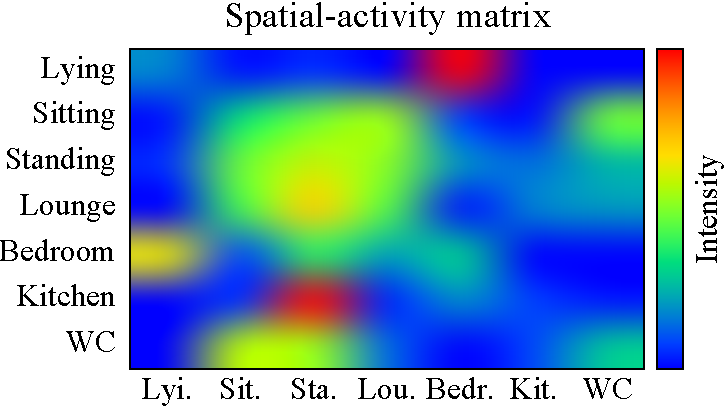
\includegraphics[width=0.50\textwidth]{chap_AAL/matrix-b-c-2}}

 \caption{Behavior matrix visualization for four normal (a,b, c, d) and two deviant days (e, f) of one person.}
 \label{fig:days}
\end{figure}

The first experiments proceeded as follows: the measurements were performed on two people aged between 25 and 32 years, with each day corresponding to a particular scenario, basically the same for each of the persons. The first, usual day represents a typical daily routine for an elderly person. It consists of sleeping, morning routine, breakfast, using toilet/household chores/reading newspaper, preparing and eating lunch, going out/watching TV/household chores/resting, dinner, watching TV/reading, and sleeping. In the second, slow day, the scenario is that the person is not feeling well and, as a consequence, is moving slowly and rests a lot. Such behavior could occur if person had the flu, heart failure, or several other general health problems, either physical or mental. In the third scenario, the person is limping due to, for example, hip pain. As a consequence, the person is also moving slowly and does not stand a lot. The person is not lying as much as on the previous day, but sits more than usual. Each person was given a loose daily scenario and an approximate timing for each activity, but performed it on her/his own. The scenarios were performed and recorded 12 times in total, consisting of eight normal days and four days where the person was not healthy. 
The length of the recordings varied between 25 and 40 minutes. Each recording/day was represented with one behavior trace.


First, we visually compared the usual-day scenario behavior traces with the slow-day and the limping-day scenario behavior traces. Figure~\ref{fig:days} represents spatio-activity matrix visualizations computed from the behavior traces of one person for the four usual days (\ref{fig:day-n-1}--\ref{fig:day-n-4}) and two deviant days (\ref{fig:day-c-1}, \ref{fig:day-c-1}). The spatio-activity matrices plotted in figures \ref{fig:day-n-1}--\ref{fig:day-n-4} captured more or less the same daily dynamics with small variations; for example, there was slightly more standing in the toilet in day~4 (\ref{fig:day-n-4}) than in day~1 (\ref{fig:day-n-1}). The slow day~(\ref{fig:day-c-1}) had an activities over location distribution (lower-right part) quite different compared from the normal days. The most significant feature is an additional orange square, which means that there was more sitting in the lounge. The distribution also deviates during a slow day (\ref{fig:day-c-2}) where, for example, the share of standing is higher than in normal days. 

The difference is even more obvious when PCA is applied. Figure~\ref{fig:PCA} shows the first three PCA components of the behavior traces plotted in Figure~\ref{fig:days}. The four circles `\textbullet' represent the usual days, while the other days are represented by crosses `$\times $'.

\begin{figure*}[t]
\centering
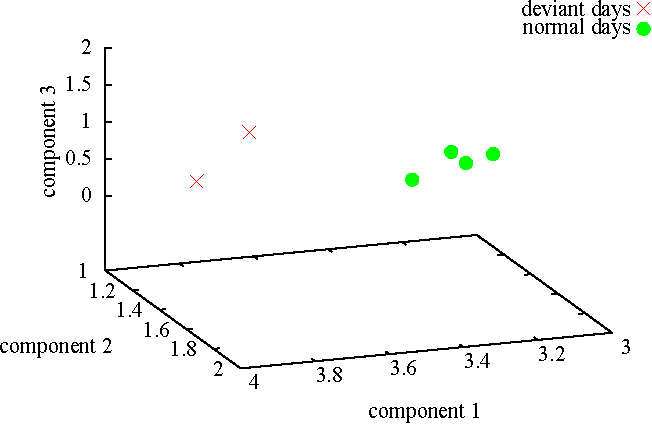
\includegraphics[width=0.8  \textwidth]{chap_AAL/PCA-plot-big}
\caption{Visualization of principal components computed from the matrices shown in Figure~\ref{fig:days}. Normal days are presented with circles, deviation days with  crosses.}
\label{fig:PCA}
\end{figure*}

The anomalous behavioral traces were computed using Algorithm~\ref{alg:LOF}, using {\it leave-one-day-out} validation; that is, one day was used for evaluation while the others were used for training. Table~\ref{tab:LOF-values} shows the LOF values for different values of $k=\{2,3\}$ for all the recordings of both persons. Normal days have $LOF < 1$ in all cases, while the anomalous days have a LOF value significantly higher than $1$.

\begin{table}[h!]
\centering
\caption{LOF values of the behavior traces. A higher value represents a higher outlierness of a behavior trace.}
\begin{tabular}{lcccc}
\toprule
 & $k$=2 & $k$=2 & $k$=3 & $k$=3 \\
Scenario & User 1 & User 2 & User 1 & User 2 \\
\hline
Normal day 1 & 0.619 & 0.615 & 0.887 & 0.963 \\
Normal day 2 & 0.694 & 0.613 & 0.904 & 0.766 \\
Normal day 3 & 0.652 & 0.639 & 0.843 & 0.797 \\
Normal day 4 & 0.601 & 0.743 & 0.832 & 0.841 \\
\hline
Limping day  & 2.369 & 4.270 & 4.519 & 6.465 \\
Slow day     & 3.274 & 2.358 & 5.451 & 4.227 \\
\toprule
\end{tabular}
\label{tab:LOF-values}
\end{table}

In the second experiment, we recorded a member of our department for a period of one month. The person was recorded during working hours, approximately eight hours per day. In this experiment, the person wore only one Ubisense chest tag. The first 10 days were used for training, while the next five days were used for evaluation. Additionally, we recorded three days when the person was experiencing some difficulties: a limping day, where the person limps while he walks; an agitation day, where person occasionally walks around the office for half a minute; and an urinary tract infection day, where the person visits toilets more than usual. In total, there were 18 working days resulting in over 90 recording hours.

The results for five regular and three anomalous days are presented in Table~\ref{tab:LOF-long} for $k={2,3,4}$. The normal working days have LOF values lower than $1$ except on the third day, while the days when the person experienced some kind of difficulty, have significantly higher LOF values.

\begin{table}[h!]
\centering
\caption{LOF values of the long-term test. A higher value represents a higher outlierness of a behavior trace.}
\begin{tabular}{lccc}
\toprule
Day & $k$=1	& $k$=2	& $k$=3 \\
\hline
Regular day 1 & 0.737 & 0.784 & 0.684	\\
Regular day 2 & 0.803 & 0.698 & 0.594	\\
Regular day 3 & 1.618 & 1.579 & 1.281	\\
Regular day 4 & 0.840 & 0.866 & 0.738	\\
Regular day 5 & 0.767 & 0.916 & 0.881	\\
\hline
Limping 		 & 3.706 & 4.820 & 6.216	\\
Agitation 	 & 7.110 & 8.987 & 12.960	\\
Urinary infection & 14.405 & 18.052 & 19.869	\\
\toprule
\end{tabular}
\label{tab:LOF-long}
\end{table}

%%%%%%%%%%%%%%%%%%%%%%%%%%%%%%%%%%%%%%%%%%%%%%%%%%%%%%%%%%%%%%%%%%%%%%%%%%%%%%%%
\section{Discussion}
\label{sec:discussion}

% more tests
%Although the initial results are promising, more realistic, long-term tests are needed to verify the performance of the newly designed method, and further improve it. However, the first results suggest that with further modifications the novel method for daily-living dynamics might prove as useful as indicated. 

% Different periods
In these experiments, we selected one day as a default unit, but in general, the approach can be applied to various period lengths. Furthermore, monitoring the behavior with different granularities by using different periods simultaneously; for example, half a day, a day, a week, or a month, would allow us to detect behavior changes that occur with different pace.

% HMM can model a single 
It should be noted that the task is based on combining activities and spatial information; therefore, applying a uniform method, such as HMMs, is not feasible. The novel method explains the two concepts by combining several existing algorithms, and specializing them for the particular task. In addition, HMMs must estimate the model learning phase parameters, whose quality depends on the labeled data amount \citep{Rabiner1989}. 

% Visulization has two functions
The spatio-activity matrix visualization can be used in two ways. First, it enables visual anomalous behavior detection; by examining the matrices, one cannotice changes in behavior dynamics. Second, it explains those cases when the automatic procedure detects anomalous behavior patterns.

% embedded sensors
The final remark concerns the type of sensors used in the experiments. Even though our approach was evaluated with wireless location sensors (that is, Ubisense), it can be applied to any sensor type from which it is possible to locate and recognize activities; for example, one can use embedded sensors as shown by \cite{Cook2012} and \cite{Storf}. 
%In fact, our future plans include an extensive experiment in an environment with embedded sensors.

%%%%%%%%%%%%%%%%%%%%%%%%%%%%%%%%%%%%%%%%%%%%%%%%%%%%%%%%%%%%%%%%%%%%%%%%%%%%%%%%
\section{Conclusion}
\label{sec:conclusion}

The main goal of this chapter was to deliver a solution whereby a caregiver can constantly and remotely observe a person's daily behavior in an efficient and unobtrusive manner. We demonstrated how to apply the unified detection framework for transforming behavior traces into a spatio-activity matrix, which captures daily behavior and presents a visualization and explanation of behavior deviations. 

We proposed a method for automatic discovery of anomalous daily behavior, which consists of feature extraction based on PCA and outlier detection implemented with the LOF algorithm. The outputs can be directly used to signal a warning to the person and caregivers, providing information that the person dynamics has changed significantly along with a relevant explanation. 
%
The experimental results showed that the proposed approach is successful in discriminating normal days from days where the person's well-being is affected. 

% FUTURE WORK
The method has not been tested thoroughly yet. Further realistic, long-term tests with the target group are needed to verify the newly designed method's performance, and to further improve it. However, the first results are quite promising; with further modifications, the novel method for daily living dynamics might prove useful as indicated. 


%%%%%%%%%%%%%%%%%%%%%%%%%%%%%%%%%%%%%%%%%%%%%%%%%%%%%%%%%%%%%%%%%%%%%%%%%%%%%%%%
%\section*{Acknowledgments}
%\label{sec:conclusion}
%This work was partly supported by the Slovenian Research Agency under the Research Programme P2-0209 Artificial Intelligence and Intelligent Systems, and partly from the European Community's Framework Programme FP7/2007-2013 under grant agreement No. 214986. We would like to thank Mitja Lu{\v s}trek, Erik Dovgan, Bo{\v z}a Cvetkovi{\' c}, Violeta Mirche\-vska for suggestions, discussions and help with the programming. 